%% !TeX root = RS.tex

\documentclass[11pt,aspectratio=169]{beamer}
\usepackage[utf8]{inputenc}
\usepackage[T1]{fontenc}
\usepackage{lmodern}
\usepackage[ngerman]{babel}
\usepackage{tikz}
\usetheme{Hannover}

\begin{document}
	\author{Joshua Bär}
	\title{FM - Bessel}
	\subtitle{}
	\logo{}
	\institute{OST Ostschweizer Fachhochschule}
	\date{16.5.2022}
	\subject{Mathematisches Seminar}
	%\setbeamercovered{transparent}
	\setbeamercovered{invisible}
	\setbeamertemplate{navigation symbols}{}
	\begin{frame}[plain]
		\maketitle
	\end{frame}
%-------------------------------------------------------------------------------	
\section{Einführung}
	\begin{frame}
		\frametitle{Frequenzmodulation}
		
		\visible<1->{
            \begin{equation} \cos(\omega_c t+\beta\sin(\omega_mt))
        \end{equation}}
		
		\only<2>{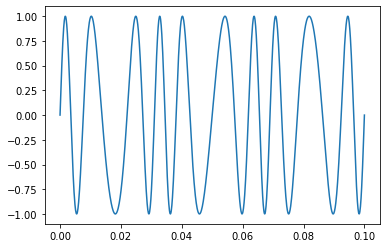
\includegraphics[scale= 0.7]{images/fm_in_time.png}}
		\only<3>{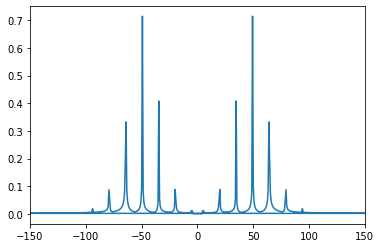
\includegraphics[scale= 0.7]{images/fm_frequenz.png}}
		\only<4>{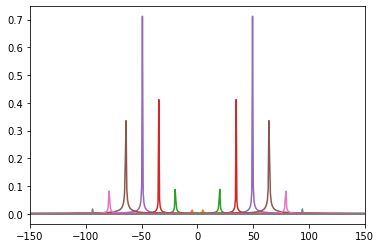
\includegraphics[scale= 0.7]{images/bessel_frequenz.png}}
		
		
	\end{frame}
%-------------------------------------------------------------------------------	
\section{Proof}
\begin{frame}
	\frametitle{Bessel}

	\visible<1->{\begin{align}
			\cos(\beta\sin\varphi)
			&=
			J_0(\beta) + 2\sum_{m=1}^\infty J_{2m}(\beta) \cos(2m\varphi)
			\\
			\sin(\beta\sin\varphi)
			&=
			J_0(\beta) + 2\sum_{m=1}^\infty J_{2m}(\beta) \cos(2m\varphi)
			\\
			J_{-n}(\beta) &= (-1)^n J_n(\beta)
		\end{align}}
	\visible<2->{\begin{align}
			\cos(A + B) 
			&= 
			\cos(A)\cos(B)-\sin(A)\sin(B)
			\\
			2\cos (A)\cos (B)
			&=
			\cos(A-B)+\cos(A+B)
			\\
			2\sin(A)\sin(B)
			&=
			\cos(A-B)-\cos(A+B)
		\end{align}}
\end{frame}

%-------------------------------------------------------------------------------	
\begin{frame}
		\frametitle{Prof->Done}
		\begin{align}
			\cos(\omega_ct+\beta\sin(\omega_mt))
			&=
			\sum_{k= -\infty}^\infty J_{k}(\beta) \cos((\omega_c+k\omega_m)t)
		\end{align}
	\end{frame}
%-------------------------------------------------------------------------------	
	\begin{frame}
	\begin{figure}
		\only<1>{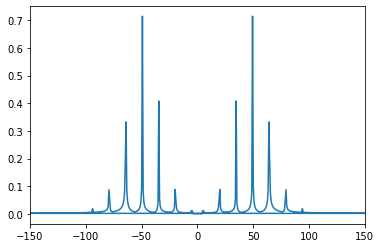
\includegraphics[scale = 0.75]{images/fm_frequenz.png}}
		\only<2>{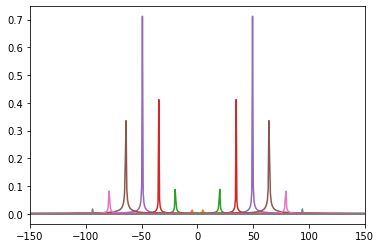
\includegraphics[scale = 0.75]{images/bessel_frequenz.png}}
	\end{figure}
	\end{frame}
%-------------------------------------------------------------------------------		
\section{Input Parameter}
	\begin{frame}
	\frametitle{Träger-Frequenz Parameter}
	\onslide<1->{\begin{equation}\cos(\omega_ct+\beta\sin(\omega_mt))\end{equation}}
	\only<1>{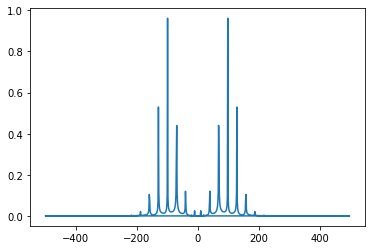
\includegraphics[scale=0.75]{images/100HZ.png}}
	\only<2>{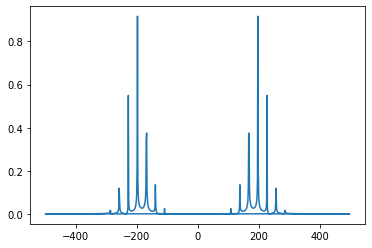
\includegraphics[scale=0.75]{images/200HZ.png}}
	\only<3>{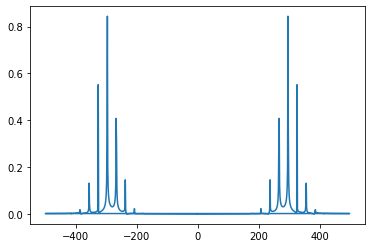
\includegraphics[scale=0.75]{images/300HZ.png}}
	\only<4>{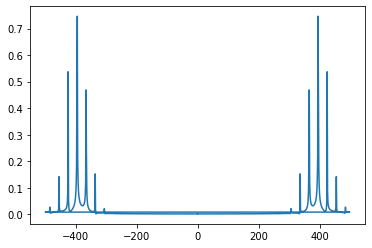
\includegraphics[scale=0.75]{images/400HZ.png}}
	\end{frame}
%-------------------------------------------------------------------------------
\begin{frame}
\frametitle{Modulations-Frequenz Parameter}
\onslide<1->{\begin{equation}\cos(\omega_ct+\beta\sin(\omega_mt))\end{equation}}
\only<1>{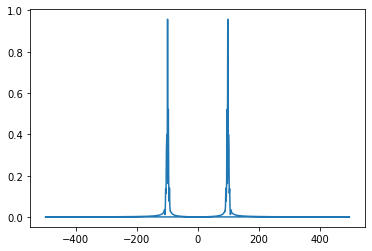
\includegraphics[scale=0.75]{images/fm_3Hz.png}}
\only<2>{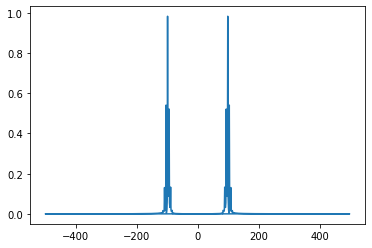
\includegraphics[scale=0.75]{images/fm_5Hz.png}}
\only<3>{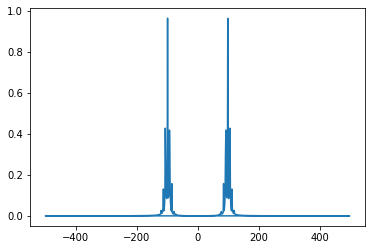
\includegraphics[scale=0.75]{images/fm_7Hz.png}}
\only<4>{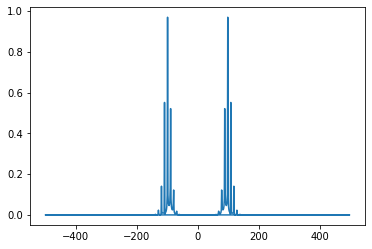
\includegraphics[scale=0.75]{images/fm_10Hz.png}}
\only<5>{\includegraphics[scale=0.75]{images/fm_20Hz.png}}
\only<6>{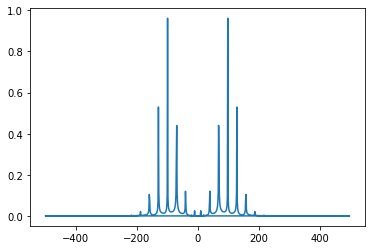
\includegraphics[scale=0.75]{images/fm_30Hz.png}}
\end{frame}	
%-------------------------------------------------------------------------------
\begin{frame}
\frametitle{Beta Parameter}
	\onslide<1->{\begin{equation}\sum_{k= -\infty}^\infty J_{k}(\beta) \cos((\omega_c+k\omega_m)t)\end{equation}}
	\only<1>{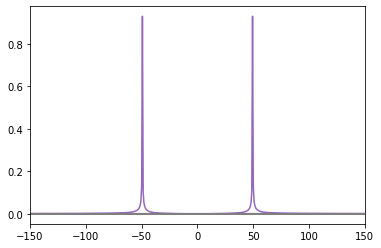
\includegraphics[scale=0.7]{images/beta_0.001.png}}
	\only<2>{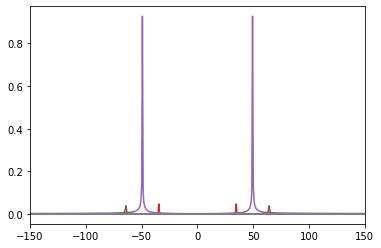
\includegraphics[scale=0.7]{images/beta_0.1.png}}
	\only<3>{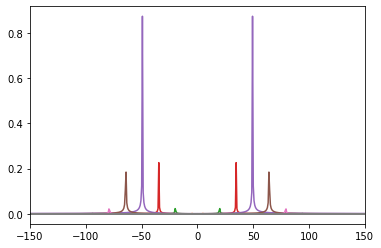
\includegraphics[scale=0.7]{images/beta_0.5.png}}
	\only<4>{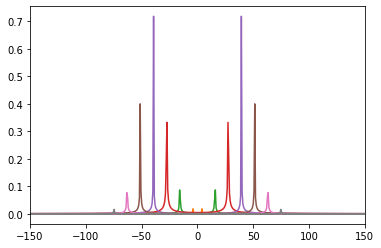
\includegraphics[scale=0.7]{images/beta_1.png}}
	\only<5>{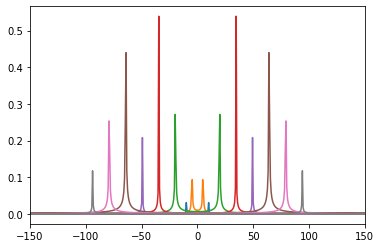
\includegraphics[scale=0.7]{images/beta_2.png}}
	\only<6>{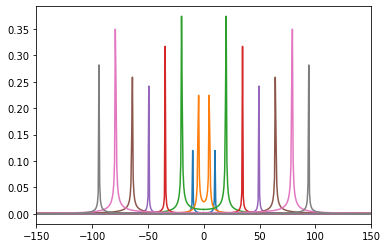
\includegraphics[scale=0.7]{images/beta_3.png}}
	\only<7>{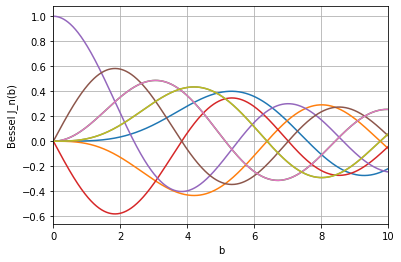
\includegraphics[scale=0.7]{images/bessel.png}}
\end{frame}	
%-------------------------------------------------------------------------------
\begin{frame}
	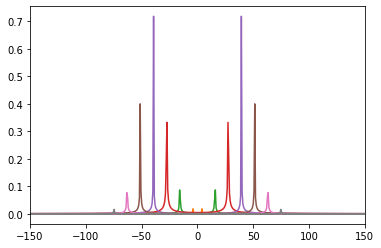
\includegraphics[scale=0.5]{images/beta_1.png}
	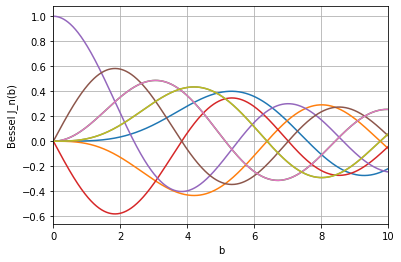
\includegraphics[scale=0.5]{images/bessel.png}
\end{frame}	
\end{document}
